\chapter{Realizacja projektu}

\section{Budowa aplikacji}

Aplikacja została stworzona przy wykorzystaniu języka \texttt{Python} w wersji \texttt{3.5}. Do sieci neuronowej wykorzystano moduł \texttt{scikit-learn} w wersji  \texttt{0.18.dev0}, zaś do zbudowania graficznego interfejsu użyto pakietu \texttt{Tkinter}.

Na aplikację składa się kilka modułów:

\begin{itemize}
    \item \texttt{main.py} - główny moduł uruchamiający aplikację.
    \item \texttt{prototype.py} - moduł testowy oraz wybierający parametry dla sieci neuronowej.
    \item \texttt{dataset.py} - importuje dane z pliku CSV i przechowuje je w wygodnej postaci.
    \item \texttt{consts.py} - zawiera parametry sieci neuronowej i inne dane.
\end{itemize}


Aby przygotować aplikację do działania, należy dodać katalog projektu do zmiennej środowiskowej \texttt{PYTHONPATH}. Można to zrobić za pomocą polecenia:

\begin{verbatim}
$ export PYTHONPATH="${PYTHONPATH}:${PWD}"
\end{verbatim}

Następnie uruchomienie aplikacji odbywa się przy użyciu komendy:

\begin{verbatim}
python3 main.py
\end{verbatim}

\newpage

\section{Zbiór uczący}
\label{zbior}

W projekcie bardzo ważny był dobór odpowiedniego zbioru uczącego jako wejście do sieci neuronowej. Wybrany został darmowy zbiór \textit{Flags Data Set} z internetowego zasobu \textit{UCI Machine Learning Repository}\footnote{http://archive.ics.uci.edu/ml/datasets/Flags}. Wybrany zestaw danych obejmuje 194 kraje z całego świata na stan z 1990 roku wraz z 30 atrybutami opisującymi cechy danego kraju jak i wygląd flagi.

Bazowy zbiór należało następnie dostosować do problemu. Przede wszystkim, trzeba było zaktualizować zbiór odejmując z niego nie istniejące już kraje oraz dodać te które doszły, na przykład kraje powstałe po upadku ZSRR bądź Jugosławii. Część krajów wprowadziła zmiany do swoich flag i je również należało poprawić. Ostatecznie zbiór wyniósł 201 krajów.

Następnie usunięto wszystkie cechy nieskorelowane z wyglądem flagi, a dokładniej: kontynent, strefa geograficzna, powierzchnia, liczba ludności, język i religia. Pozostały \textbf{23} cechy:

\begin{itemize}
    \item \texttt{bars} - Liczba pionowych pasów
    \item \texttt{stripes} - Liczba poziomych pasów
    \item \texttt{colours} - Liczba różnych kolorów
    \item \texttt{red, green, blue, gold, white, black, orange} - Czy występuje kolor czerwony, zielony, niebieski, złoty, biały, czarny, pomarańczowy
    \item \texttt{mainhue} - Dominujący kolor na fladze
    \item \texttt{circles} - Liczba okręgów
    \item \texttt{crosses} - Liczba pionowych krzyży
    \item \texttt{saltires} - Liczba krzyży św. Andrzeja
    \item \texttt{quarters} - Liczba ćwiartek
    \item \texttt{sunstars} - Liczba symboli Słońca lub gwiazdy
    \item \texttt{crescent} - Czy występuje półksiężyc
    \item \texttt{triangle} - Czy występuje trójkąt
    \item \texttt{icon} - Czy występuje element nieożywiony (symbol/emblemat)
    \item \texttt{animate} - Czy występuje element ożywiony (zwierzę/roślina/człowiek)
    \item \texttt{text} - Czy występuje tekst
    \item \texttt{topleft} - Dominujący kolor w lewym górnym rogu
    \item \texttt{botright} - Dominujący kolor w prawym dolnym
\end{itemize}

\newpage

\section{Badania}

Badania sieci neuronowej przeprowadzono w celu sprawdzenia jakie wartości parametrów sprawdzają się najlepiej dla rozpatrywanego zagadnienia, oraz aby zbadać wpływ zbioru wejściowego na efektywność algorytmu. Badania rozpoczęto od zbudowania sieci neuronowej. Wybrano prosty perceptron wielowarstwowy bazujący na uczeniu nadzorowanym i jako jego realizację wybrano klasyfikator \texttt{MLPClassifier}.

Następnie wybrano odpowiednie współczynniki posługując się wiedzą nabytą na poprzednich kursach oraz testując efektywność algorytmu dla różnych wartości danego parametru z zadanego przedziału przy stałych innych współczynnikach. Ostateczne wartości parametrów przedstawia poniższa tabela \ref{tab:params}.

\begin{table}[h!]
    \centering
    \caption{Parametry algorytmów.}
    \label{tab:params}
    \begin{tabular}{p{3cm}p{3cm}p{9cm}}
        \toprule
        \textbf{Parametr} & \textbf{Wartość} & \textbf{Opis} \\
        \midrule
        \texttt{algorithm} & \texttt{l-bfgs} & Algorytm działania (\textit{quasi-Newton method}). \\
        \texttt{max\_iter} & \texttt{500} & Maksymalna liczba iteracji. \\
        \texttt{alpha} & \texttt{0.88} & Parametr regularyzacji. \\
        \texttt{learning\_rate} & \texttt{constant} & Tempo uczenia. \\
        \texttt{activation} & \texttt{logistic} & Funkcja aktywacji algorytmu. \\
        \bottomrule
    \end{tabular}
\end{table}

W kolejnym kroku przeprowadzono testy mające na celu dobranie odpowiedniej liczby warstw ukrytych oraz liczby neuronów w każdej. Badania wykonano zarówno dla zbioru bazowego, bez przeprowadzonych modyfikacji opisanych w rozdziale \ref{zbior}, jak i dla zbioru przerobionego. Stwierdzono, że usunięcie zbędnych danych pozwoliło na znaczący wzrost efektywności nauczonej sieci.

Efektywność algorytmu sprawdzano testując go na tym samym zbiorze, na którym został nauczony poprzez liczenie liczby poprawnych odpowiedzi, którą to następnie dzielono przez całkowitą liczbę instancji, otrzymując tym samym procentowy wskaźnik.

Dla zbioru bazowego zastosowano jedną oraz dwie warstwy ukryte, gdzie dla każdej z nich przetestowano liczbę neuronów z przedziału $\langle1, 25\rangle$. Wyniki testu pokazały, że największą efektywność wynoszącą \textbf{63.4\%} uzyskano dla 15 oraz 18 neuronów dla odpowiednio pierwszej i drugiej warstwy ukrytej.

\begin{lstlisting}[caption=Wynik badań dla zbioru bazowego]
Highest score:
1st hidden layer size: 15
2nd hidden layer size: 18
Number of correct answers: 123
Total number of questions: 194
Effectiveness: 63.4%
\end{lstlisting}

\newpage

Wynik efektywności algorytmu dla przeprowadzonego testu nie był zadowalający, dlatego też przeprowadzono badanie dla zbioru zmodyfikowanego z usuniętymi nieskorelowanymi danymi. Wyniki pokazały, że aby osiągnąć dużą dokładność wystarczy tylko jedna warstwa ukryta i już przy 3 neuronach udało się osiągnąć większą efektywność niż dla zbioru bazowego. Od 7 neuronów udało się otrzymać dokładność rzędu \textbf{95.0\%} i była ona od tego momentu stała przy zwiększaniu liczby neuronów. 7 neuronów zastosowano zatem do klasyfikatora do finalnej wersji aplikacji.

\begin{lstlisting}[caption=Wynik badań dla zbioru zmodyfikowanego]
Highest score:
1st hidden layer size: 7
Number of correct answers: 191
Total number of questions: 201
Effectiveness: 95.0%
\end{lstlisting}

\begin{table}[ht!]
\centering
\caption{Procentowa dokładność dla różnych wartości neuronów w jednej warstwie ukrytej}
\label{score}
\begin{tabular}{@{}|c|c|c|c|c|c|c|c|c|c|c|@{}}
\toprule
\textbf{Liczba neuronów}  & 1    & 2    & 3    & 4    & 5    & 6    & 7    & 8    & 9    & 10   \\ \midrule
\textbf{Efektywność (\%)} & 10.4 & 42.8 & 84.1 & 93.0 & 94.5 & 94.5 & 95.0 & 95.0 & 95.0 & 95.0 \\ \bottomrule
\end{tabular}
\end{table}

\begin{figure}[h!]
	\centering
	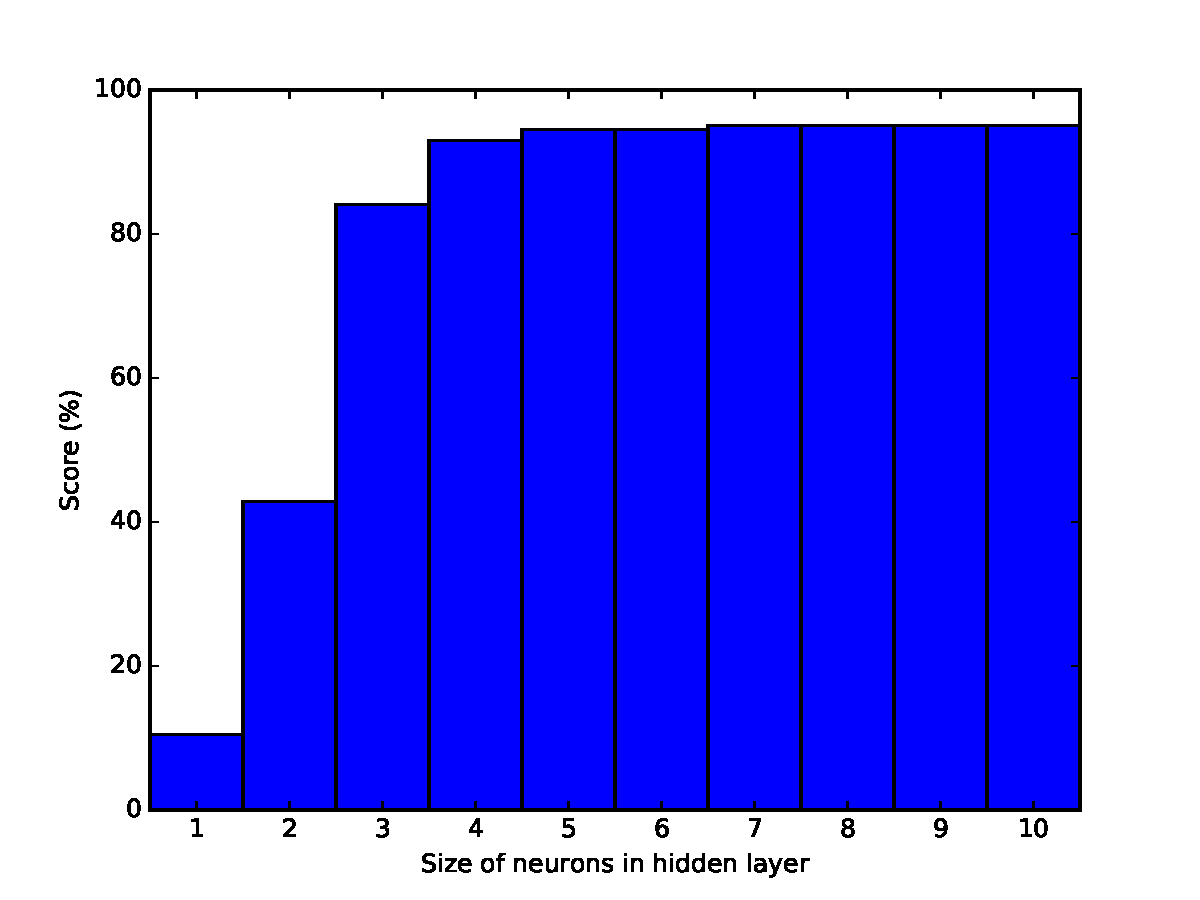
\includegraphics[width=0.95\linewidth]{hidden_sizes.pdf}
	\label{hidden_sizes}
	\caption{Wpływ liczby neuronów w jednej warstwie ukrytej na efektywność algorytmu}
\end{figure}

\newpage

Nauczony algorytm radził sobie bardzo dobrze z odgadywaniem państw, gdyż większość z nich odgadywana była z ponad 90\% prawdopodobieństwem (do testu w dalszym ciągu używano zbioru wejściowego), co zbadano za pomocą funkcji \texttt{predict\_proba} udostępnioną przez klasyfikator, która to ukazuje procentowy rozkład pewności klasyfikacji wszystkich klas. Dla sprawdzenia wybierane były 3 klasy z najwyższą pewnością.

\begin{lstlisting}[caption=Przykładowy rozkład pewności klas dla dla poprawnego wskazania państwa Nepal]
Country: Nepal
1st probability: 94.0% of country: Nepal
2nd probability: 2.0% of country: Italy
3rd probability: 1.8% of country: Israel
\end{lstlisting}

Uprzednie testy wykazały 95.0\% efektywność przy odgadywaniu, dlaczego więc nie udało się osiągnąć 100\%? Jest to związane z tym, że część flag różnych krajów jest identyczna, bądź bardzo do siebie podobna i cechy jakimi były one określane okazały się identyczne. Sprawiło to, że algorytm oznaczał z takim samym prawdopodobieństwem wystąpienie i jednego i drugiego kraju, co spowodowało obniżenie ogólnej efektywności. Przykładami takich krajów są chociażby Luksemburg i Holandia czy Indonezja i Maroko.

\begin{lstlisting}[caption=Przykładowy rozkład pewności klas dla niepoprawnego wskazania Szwajcarii]
Country: Switzerland
1st probability: 35.9% of country: Denmark
2nd probability: 35.9% of country: Switzerland
3rd probability: 5.4% of country: Norway
\end{lstlisting}

Po badaniach efektywności nauczonego algorytmu, sprawdzono również czasy uczenia dla różnej liczby neuronów w warstwie ukrytej. Stwierdzono, że czas uczenia rośnie ze złożonością zbliżoną do stałej, oraz potwierdziły słuszność wybrania 7 neuronów, gdyż stosunek jakości algorytmu do czasu jego nauczania był najbardziej optymalny. Nie było sensu zatem wybierania wyższej liczby, gdyż efektywność dla nich była taka sama jak dla 7, zaś czasy uczenia rosły.

\begin{table}[ht!]
\centering
\caption{Czasy uczenia dla różnych wartości neuronów w jednej warstwie ukrytej}
\label{times}
\begin{tabular}{@{}|c|c|c|c|c|c|c|c|c|c|c|@{}}
\toprule
\textbf{Liczba neuronów}  & 1    & 2    & 3    & 4    & 5    & 6    & 7    & 8    & 9    & 10  \\ \midrule
\textbf{Czas uczenia (s)} & 5.77 & 5.83 & 6.03 & 6.09 & 6.19 & 6.26 & 6.21 & 6.51 & 6.49 & 6.9 \\ \bottomrule
\end{tabular}
\end{table}

\newpage

\begin{figure}[h!]
	\centering
	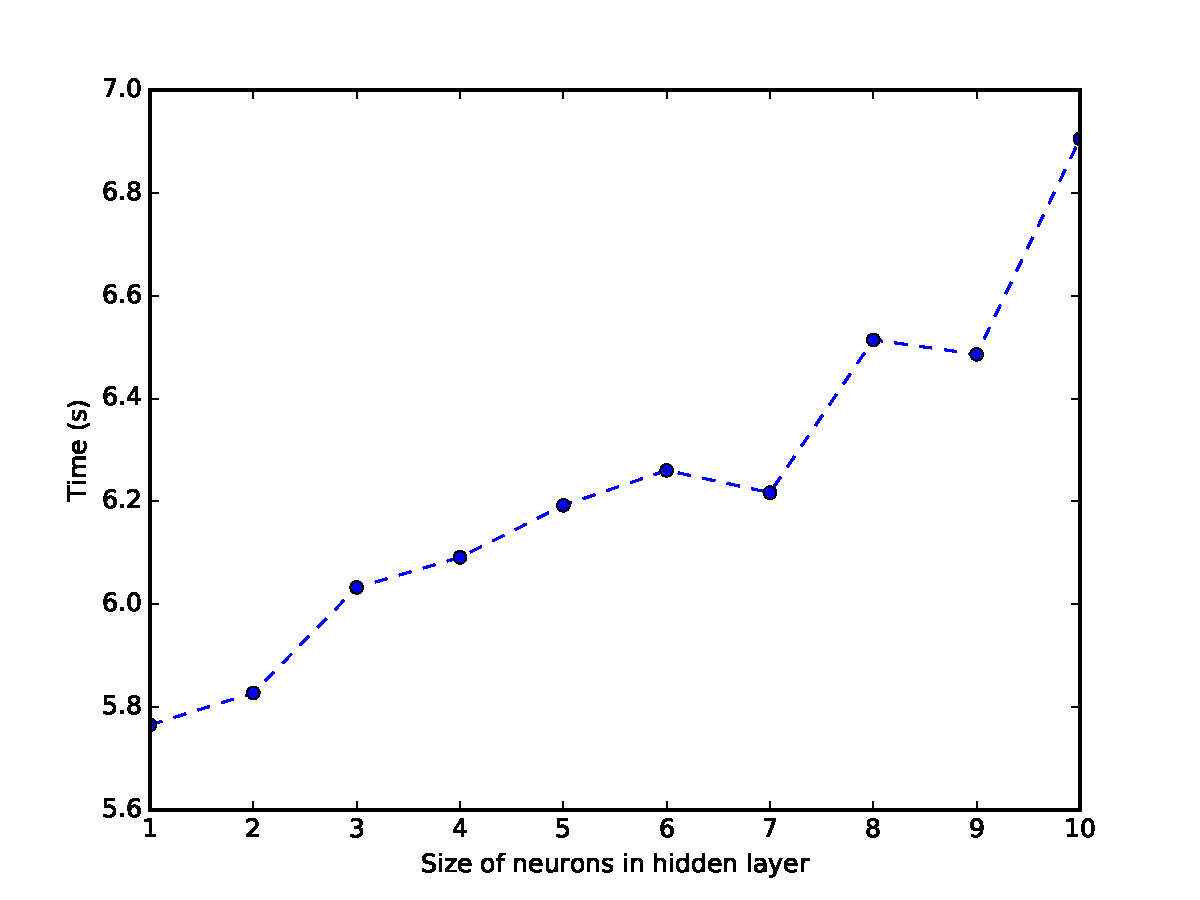
\includegraphics[width=0.90\linewidth]{times.pdf}
	\label{features}
	\caption{Wykres czasów uczenia dla różnych wartości neuronów w jednej warstwie ukrytej}
\end{figure}

Do tej pory wszystkie badania przeprowadzano testując algorytm na tym samym zestawie danych, na którym był on uczony. Postanowiono sprawdzić jakie uzyska się wyniki gdy zestaw zostanie odpowiednio zdywersyfikowany. Dla każdej z 201 próbek losowo wybrano 2 z 23 cech, które zmodyfikowano tak, że gdy cecha miała wartość $>0$, zmieniano ją na 0, zaś dla 0 ustawiano wartość 1. Operację wykonano po 10 razy dla każdej klasy, za każdym razem zapisując jako nową próbkę, co poskutkowało wytworzeniem zbioru o wielkości 2010 próbek. Następnie przeprowadzono testy odpowiednio zmieniając zbiory podczas uczenia oraz testowania.

\begin{table}[ht!]
\centering
\caption{Porównanie efektywności uczenia dla różnych zbiorów uczących i testowych}
\label{comparison}
\resizebox{\textwidth}{!}{%
\begin{tabular}{@{}|c|c|c|c|c|c|@{}}
\toprule
\textbf{Zbiór uczący}     & Bazowy        & Bazowy        & Wygenerowany  & Wygenerowany  & Wygenerowany      \\ \midrule
\textbf{Zbiór testowy}    & Bazowy        & Wygenerowany  & Wygenerowany  & Bazowy        & Inny wygenerowany \\ \midrule
\textbf{Efektywność (\%)} & \textbf{95.0} & \textbf{64.7} & \textbf{82.4} & \textbf{91.0} & \textbf{65.1}     \\ \bottomrule
\end{tabular}%
}
\end{table}

Jak widać po wynikach przeprowadzonych testów, żaden test nie zbliżył się do efektywności, jaką cechuje testowanie na bazowym zbiorze uczącym, czyli 95\%. Jednakże czynione jest tutaj założenie, że gracz odpowie poprawnie na wszystkie pytania. Sprawdzenie na zbiorze wygenerowanym, czyli takim, w którym założone są pomyłki, cechuje się niestety bardzo niską efektywnością wynoszącą 64.7\%. Testując na zbiorze wygenerowanym o wiele lepiej radzi sobie algorytm nauczony bezpośrednio na nim samym, jednakże nie jest to również zadowalająca efektywność, zaś testowanie go innym zbiorem wygenerowanym powoduje znowuż znaczny spadek efektywności. Do finalnej wersji aplikacji przeznaczono zatem algorytm nauczony na bazowej, niezdywersyfikowanej wersji zbioru.

\newpage

Na koniec, postanowiono sprawdzić, które atrybuty najbardziej przysłużyły się do poprawnego odgadywania flag. Pozwoliło to odpowiednio ułożyć pytania w kolejności od najbardziej przydatnych do najmniej, zgodnie z przewidywanym zaangażowaniem gracza w poprawne odgadywanie na zadawane pytania, gdzie na początku zdolność skupienia gracza jest najwyższa, zaś po otrzymaniu serii pytań, jego odpowiedzi są przeważnie mniej dokładne.

Do wyboru przydatności atrybutów posłużono się selekcją cech, która jest udostępniona metodą \texttt{SelectKBest} wybierającą k-najlepszych cech. Wygenerowano zdywersyfikowany zbiór, następnie wybrano $k=\langle1, 23\rangle$ najlepszych cech i dodano do siebie częstość występowania danej cechy. Testy przeprowadzono 20 razy, za każdym razem generując nowy zbiór, zaś wyniki uśredniono.

\begin{table}[ht!]
\centering
\caption{Selekcja cech 1/2}
\label{selection1}
\resizebox{\textwidth}{!}{%
\begin{tabular}{|c|c|c|c|c|c|c|c|c|c|c|c|c|}
\hline
\textbf{Atrybut}  & sunstars & stripes & bars & botright & mainhue & topleft & gold & green & blue & crosses & circles & white \\ \hline
\textbf{Selekcja} & 436      & 418     & 405  & 366      & 360     & 351     & 296  & 283   & 281  & 261     & 235     & 202   \\ \hline
\end{tabular}%
}
\end{table}

\begin{table}[ht!]
\centering
\caption{Selekcja cech 2/2}
\label{selection2}
\resizebox{\textwidth}{!}{%
\begin{tabular}{|c|c|c|c|c|c|c|c|c|c|c|c|}
\hline
\textbf{Atrybut}  & icon & black & quarters & red & colours & animate & triangle & orange & saltires & text & crescent \\ \hline
\textbf{Selekcja} & 189  & 186   & 180      & 152 & 130     & 126     & 73       & 70     & 38       & 21   & 1        \\ \hline
\end{tabular}%
}
\end{table}

\begin{figure}[h!]
	\centering
	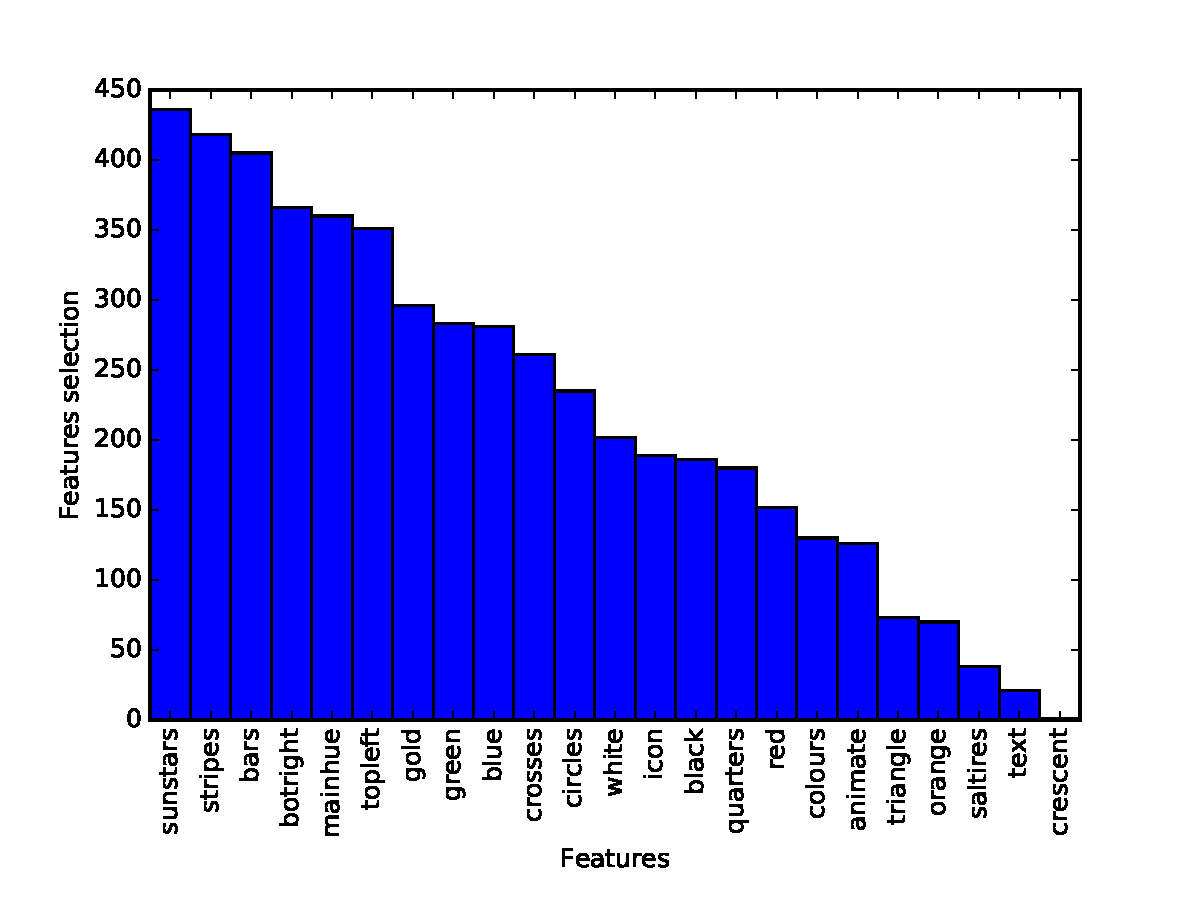
\includegraphics[width=0.95\linewidth]{features.pdf}
	\label{features}
	\caption{Posortowany ranking cech}
\end{figure}

\section{Opis interfejsu i przebiegu aplikacji}

Zgodnie z założeniami dla aplikacji zbudowano graficzny interfejs ułatwiający interakcję gracza z komputerem. Po uruchomieniu programu, pojawia się główne okno, w którym wybrać możemy rozpoczęcie rozgrywki bądź zakończenie działania.

\begin{figure}[h!]
	\centering
	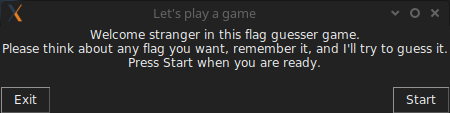
\includegraphics[width=0.7\linewidth]{main_window.png}
	\label{main-window}
	\caption{Główne okno}
\end{figure}

Po rozpoczęciu wyświetlać się będą po kolei pytania dotyczące każdej z cech nauczonego zbioru. Pytania dzielą się na 3 typy: okno wyboru liczby, koloru, bądź prawda/fałsz. Dla ułatwienia można odpowiadać przesuwając odpowiedzi strzałkami góra/dół i zatwierdzając odpowiedź po wciśnięciu klawisza ENTER.

\begin{figure}[h!]
	\centering
	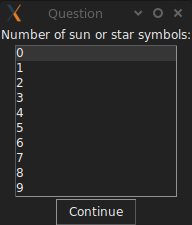
\includegraphics[width=0.28\linewidth]{q1.png}
	\label{q1}
	\caption{Okno wyboru liczby}
\end{figure}

\begin{figure}[h!]
	\centering
	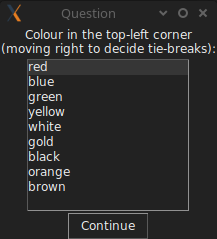
\includegraphics[width=0.3\linewidth]{q2.png}
	\label{q2}
	\caption{Okno wyboru koloru}
\end{figure}

\newpage

\begin{figure}[h!]
	\centering
	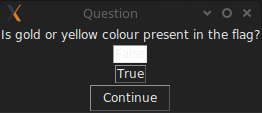
\includegraphics[width=0.4\linewidth]{q3.png}
	\label{q3}
	\caption{Okno wyboru prawda/fałsz}
\end{figure}

Wyświetlanie 23 pytań podzielone jest na 4 sekcje, gdzie co 6 pytań wyświetlane jest zapytanie czy gracz nie ma na myśli państwa, które znajduje się w tym momencie na pierwszym miejscu według rozkładu pewności. Dzięki ułożeniu pytań względem rankingu cech istnieje możliwość odgadnięcia państwa bez przechodzenia przez wszystkie państwa. Cechy, które jeszcze nie pojawiły się w pytaniach ustawiane są na 0.

\begin{figure}[h!]
	\centering
	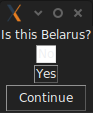
\includegraphics[width=0.15\linewidth]{flag.png}
	\label{flag}
	\caption{Okno pytania o flagę}
\end{figure}

W momencie, gdy algorytm niepoprawnie odgadł państwo, aplikacja przechodzi do zadawania kolejnych pytań, bądź po przejściu przez wszystkie, przedstawia propozycję kolejnego państwa znajdującego się na kolejnej pozycji w rozkładzie pewności. Po odgadnięciu państwa wyświetlane jest okno końcowe, przedstawiające informację o tym ile pytań zostało do tej pory zadanych oraz ile prób zajęło zgadnięcie flagi.

\begin{figure}[h!]
	\centering
	
\includegraphics[width=0.9\linewidth]{finish.png}
	\label{finish}
	\caption{Okno końcowe}
\end{figure}

Po zamknięciu okna końcowego aplikacja wraca do menu głównego, z którego można rozpocząć kolejną rozgrywkę.